% Options for packages loaded elsewhere
\PassOptionsToPackage{unicode}{hyperref}
\PassOptionsToPackage{hyphens}{url}
%
\documentclass[
]{article}
\usepackage{lmodern}
\usepackage{amssymb,amsmath}
\usepackage{ifxetex,ifluatex}
\ifnum 0\ifxetex 1\fi\ifluatex 1\fi=0 % if pdftex
  \usepackage[T5]{fontenc}
  \usepackage[utf8]{inputenc}
  \usepackage[vietnamese]{babel}
  \usepackage{textcomp} % provide euro and other symbols
\else % if luatex or xetex
  \usepackage{unicode-math}
  \usepackage[vietnamese]{babel}
  \defaultfontfeatures{Scale=MatchLowercase}
  \defaultfontfeatures[\rmfamily]{Ligatures=TeX,Scale=1}
\fi
% Use upquote if available, for straight quotes in verbatim environments
\IfFileExists{upquote.sty}{\usepackage{upquote}}{}
\IfFileExists{microtype.sty}{% use microtype if available
  \usepackage[]{microtype}
  \UseMicrotypeSet[protrusion]{basicmath} % disable protrusion for tt fonts
}{}
\makeatletter
\@ifundefined{KOMAClassName}{% if non-KOMA class
  \IfFileExists{parskip.sty}{%
    \usepackage{parskip}
  }{% else
    \setlength{\parindent}{0pt}
    \setlength{\parskip}{6pt plus 2pt minus 1pt}}
}{% if KOMA class
  \KOMAoptions{parskip=half}}
\makeatother
\usepackage{xcolor}
\IfFileExists{xurl.sty}{\usepackage{xurl}}{} % add URL line breaks if available
\IfFileExists{bookmark.sty}{\usepackage{bookmark}}{\usepackage{hyperref}}
\hypersetup{
  hidelinks,
  pdfcreator={LaTeX via pandoc}}
\urlstyle{same} % disable monospaced font for URLs
\usepackage{longtable,booktabs}
% Correct order of tables after \paragraph or \subparagraph
\usepackage{etoolbox}
\makeatletter
\patchcmd\longtable{\par}{\if@noskipsec\mbox{}\fi\par}{}{}
\makeatother
% Allow footnotes in longtable head/foot
\IfFileExists{footnotehyper.sty}{\usepackage{footnotehyper}}{\usepackage{footnote}}
\makesavenoteenv{longtable}
\usepackage{graphicx}
\makeatletter
\def\maxwidth{\ifdim\Gin@nat@width>\linewidth\linewidth\else\Gin@nat@width\fi}
\def\maxheight{\ifdim\Gin@nat@height>\textheight\textheight\else\Gin@nat@height\fi}
\makeatother
% Scale images if necessary, so that they will not overflow the page
% margins by default, and it is still possible to overwrite the defaults
% using explicit options in \includegraphics[width, height, ...]{}
\setkeys{Gin}{width=\maxwidth,height=\maxheight,keepaspectratio}
% Set default figure placement to htbp
\makeatletter
\def\fps@figure{htbp}
\makeatother
\setlength{\emergencystretch}{3em} % prevent overfull lines
\providecommand{\tightlist}{%
  \setlength{\itemsep}{0pt}\setlength{\parskip}{0pt}}
\setcounter{secnumdepth}{-\maxdimen} % remove section numbering

\author{}
\date{}

\begin{document}

TRƯỜNG ĐẠI HỌC SƯ PHẠM TP.HỒ CHÍ MINH

KHOA CÔNG NGHỆ THÔNG TIN


\includegraphics[width=3.54167in,height=1.78506in]{./media/image1.png}

TIỂU LUẬN MÔN HỌC

\textbf{BÁO CÁO THỰC HÀNH NGHỀ NGHIỆP}

Đề tài: TỔNG HỢP NỘI DUNG HỌC TẬP -- ĐỊNH HƯỚNG NGHỀ NGHIỆP -- KỸ NĂNG
SỐ

\textbf{Giảng viên hướng dẫn:}

\begin{enumerate}
\def\labelenumi{\arabic{enumi}.}
\item
  CN. \textbf{Lê Thanh Thoại}
\end{enumerate}

\begin{quote}
\textbf{Sinh viên thực hiện:}

Họ tên: Nguyễn Trần Nam Khánh

MSSV: 49.01.104.070

Lớp: 49.01.CNTT.D
\end{quote}

\textbf{Lời cam đoan}

Tôi xin cam đoan rằng toàn bộ nội dung trong báo cáo này là kết quả của
quá trình học tập và nghiên cứu nghiêm túc của bản thân dưới sự hướng
dẫn của các giảng viên bộ môn. Các số liệu, kết quả và trích dẫn trong
báo cáo đều được ghi rõ nguồn gốc. Tôi hoàn toàn chịu trách nhiệm trước
pháp luật nếu có bất kỳ sai phạm nào liên quan đến tính trung thực của
nội dung trong báo cáo này.

\emph{Thành phố Hồ Chí Minh, ngày Ngày 17 tháng 5 năm 2026}

\emph{Ký tên}

\emph{Nguyễn Trần Nam Khánh}

\emph{\hfill\break
}

\textbf{Tóm tắt báo cáo}

Báo cáo này trình bày tổng quan về quá trình tự học và định hướng nghề
nghiệp cá nhân trong giai đoạn giữa kỳ của học phần \textbf{Thực hành
nghề nghiệp}. Nội dung báo cáo tập trung vào việc làm chủ các kỹ năng số
nền tảng (Linux, Git, LaTeX), thiết lập lộ trình phát triển bản thân
hướng tới vị trí \textbf{Kỹ sư Mạng/Hệ thống}, và xây dựng bộ hồ sơ năng
lực số (LinkedIn, Portfolio, CV). Kết quả đạt được là một nền tảng kỹ
thuật vững chắc để chuẩn bị cho các dự án đồ án và thực tập thực tế
trong tương lai.

\textbf{Chương 1:} Giới thiệu cá nhân \& Mục tiêu nghề nghiệp

\textbf{1.1 Thông tin sinh viên}

\begin{itemize}
\item
  \textbf{Họ tên:} Nguyễn Trần Nam Khánh
\item
  \textbf{Mã số sinh viên:} 49.01.104.070
\item
  \textbf{Chuyên ngành:} Công nghệ thông tin
\item
  \textbf{Khoá học:} 2023 -- 2027
\end{itemize}

\textbf{1.2 Lý do chọn ngành}

Lý do tôi lựa chọn theo học ngành Công nghệ thông tin xuất phát từ niềm
đam mê tìm hiểu cách thức vận hành của các hệ thống máy tính và mạng máy
tính. Thay vì tập trung hoàn toàn vào việc phát triển phần mềm, tôi nhận
thấy mình có thế mạnh và sự hứng thú đặc biệt trong việc chẩn đoán, xử
lý sự cố kỹ thuật (troubleshooting) và tối ưu hóa hệ thống phần cứng,
phần mềm.

Đồng thời, tôi là một người thích giao tiếp và mong muốn dùng kiến thức
CNTT của mình để hỗ trợ, giải quyết các rào cản công nghệ cho người
dùng, giúp tối ưu hóa hiệu suất làm việc của doanh nghiệp. Vì vậy, tôi
chọn ngành này để xây dựng nền tảng vững chắc cho định hướng trở thành
một chuyên viên IT Support/Helpdesk chuyên nghiệp.

\textbf{1.3 Định hướng nghề nghiệp dự kiến}

\textbf{Vị trí khởi đầu:} Trở thành Chuyên viên Hỗ trợ Kỹ thuật
(\textbf{IT Support Engineer / IT Helpdesk}) tại các doanh nghiệp hoặc
các đơn vị cung cấp dịch vụ Managed Services. Tập trung vào việc quản lý
thiết bị đầu cuối (End-user devices), hỗ trợ kỹ thuật cho người dùng,
quản trị hệ thống mạng nội bộ doanh nghiệp và xử lý các sự cố phần
cứng/phần mềm cơ bản đến nâng cao.

\textbf{Lộ trình phát triển dài hạn (Sau 3--5 năm):} Từ nền tảng IT
Support, định hướng phát triển chuyên sâu lên các vị trí quản trị và tối
ưu hóa hạ tầng công nghệ của doanh nghiệp như Quản trị viên hệ thống
(\textbf{System Administrator}) hoặc Quản trị viên mạng (\textbf{Network
Administrator}).

\textbf{1.4 Mục tiêu ngắn hạn (6 -- 12 tháng)}

\textbf{Về học tập và tốt nghiệp:}

\begin{itemize}
\item
  Hoàn thành chương trình đào tạo để tốt nghiệp đúng hạn.
\item
  Củng cố vững chắc các kiến thức nền tảng trường học về Mạng máy tính
  (TCP/IP, DHCP, DNS), Hệ điều hành (Windows Server, Linux) và Phần cứng
  máy tính.
\end{itemize}

\textbf{Về chứng chỉ nghề nghiệp và kỹ năng chuyên môn:}

\begin{itemize}
\item
  Tự học và phấn đấu đạt được ít nhất một chứng chỉ quốc tế nền tảng về
  IT Support / Network (Ví dụ: \emph{CompTIA A+, Google IT Support
  Professional}, hoặc hoàn thành khóa học \emph{CCNA}).
\item
  Rèn luyện kỹ năng thực hành cấu hình thiết bị mạng (Router, Switch),
  quản trị hệ thống tài khoản người dùng (Active Directory) thông qua
  các bài Lab thực tế.
\end{itemize}

\textbf{Về phát triển kỹ năng mềm:}

\begin{itemize}
\item
  Nâng cao năng lực tiếng Anh chuyên ngành để đọc hiểu tài liệu kỹ
  thuật, tra cứu lỗi (troubleshoot) trên các diễn đàn công nghệ quốc tế
  và giao tiếp cơ bản với người dùng nước ngoài.
\item
  Trau dồi kỹ năng giao tiếp, lắng nghe và giải quyết vấn đề để có thể
  tiếp nhận và xử lý yêu cầu của người dùng một cách chuyên nghiệp, bình
  tĩnh.
\end{itemize}

\textbf{Về cơ hội việc làm:}

\begin{itemize}
\item
  Tìm kiếm và ứng tuyển thành công vào vị trí \textbf{Thực tập sinh IT
  Support / Helpdesk} tại một doanh nghiệp hoặc công ty dịch vụ công
  nghệ để tích lũy kinh nghiệm thực tế trước khi tốt nghiệp.
\end{itemize}

\textbf{Chương 2:} Digital Skills \& Kỹ năng nền tảng

Trong lộ trình phát triển trở thành một kỹ sư CNTT, việc làm chủ các
công cụ hỗ trợ và kỹ năng số là nền tảng quan trọng giúp tối ưu hóa hiệu
suất làm việc. Chương này trình bày các kỹ năng tôi đã tích lũy và ứng
dụng thực tế trong quá trình học tập.

\textbf{2.1 Quản lý mã nguồn với Git \& Github}

Qua việc thực hiện nhiều dự án tiểu luận và đồ án môn học, tôi đã hình
thành thói quen làm việc chuyên nghiệp với hệ thống quản lý phiên bản
Git.

\begin{itemize}
\item
  Trải nghiệm: Tôi đã thuần thục các thao tác cơ bản nhưng cốt lõi như
  commit để ghi lại các mốc thay đổi, push để đẩy dữ liệu lên kho lưu
  trữ trực tuyến và pull để đồng bộ hóa mã nguồn về máy cá nhân. Việc
  này giúp tôi loại bỏ hoàn toàn rủi ro mất mát dữ liệu hoặc nhầm lẫn
  giữa các phiên bản bài làm.
\item
  Xây dựng thương hiệu cá nhân: Đặc biệt, tôi đã triển khai thành công
  \textbf{GitHub Pages}. Thay vì chỉ lưu trữ mã nguồn ẩn, tôi sử dụng
  công cụ này để xây dựng một trang \textbf{Portfolio/CV online}. Đây
  không chỉ là nơi lưu trữ các dự án đã qua mà còn là một bộ hồ sơ năng
  lực trực quan, giúp nhà tuyển dụng và giảng viên có cái nhìn chuyên
  nghiệp về lộ trình phát triển của bản thân.
\end{itemize}

\textbf{2.2 Soạn thảo văn bản học thuật với LaTeX}

Thay vì sử dụng các công cụ truyền thống như \textbf{Microsoft Word},
tôi chuyển sang sử dụng \textbf{LaTeX} cho các báo cáo quan trọng liên
quan đến ngành CNTT.

\begin{itemize}
\item
  Trải nghiệm thực tế: Tôi đã tự thiết lập môi trường làm việc cục bộ
  (local) với MiKTeX và TeXstudio. Việc soạn thảo bằng mã lệnh giúp tôi
  kiểm soát tuyệt đối định dạng của văn bản, từ các công thức toán học
  phức tạp đến việc quản lý mục lục tự động.
\item
  Sự tiện lợi: Điểm vượt trội lớn nhất là khả năng kết hợp giữa LaTeX và
  GitHub. Mọi thay đổi trong báo cáo đều được quản lý như một dự án phần
  mềm, cho phép tôi kiểm tra lại lịch sử chỉnh sửa một cách nhanh chóng
  và tiện lợi hơn rất nhiều so với cách lưu trữ tệp tin thông thường.
\end{itemize}

\textbf{2.3 Công cụ cộng tác và Quản lý công việc}

Để duy trì tiến độ học tập và làm việc nhóm hiệu quả, tôi tận dụng hệ
sinh thái Google Workspace làm trung tâm phối hợp:

\begin{itemize}
\item
  Google Docs: Được sử dụng trong giai đoạn khởi tạo, giúp các thành
  viên trong nhóm cùng nhau lên ý tưởng (brainstorming) và phác thảo nội
  dung sơ bộ một cách trực tiếp theo thời gian thực.
\item
  Google Sheets: Đóng vai trò là công cụ quản trị dự án thu nhỏ. Tôi sử
  dụng trang tính để phân chia nhiệm vụ cụ thể cho từng thành viên,
  thiết lập thời hạn (deadline) và theo dõi tiến độ hoàn thành thông qua
  các biểu đồ trực quan.
\item
  Google Calendar: Đây là công cụ điều phối thời gian chủ chốt. Tôi sử
  dụng lịch để lên lịch trình học tập, nhắc hẹn các buổi họp nhóm và đặc
  biệt là đánh dấu các mốc báo cáo hàng tuần để đảm bảo không bỏ lỡ các
  đầu mục công việc quan trọng.
\end{itemize}

\textbf{Chương 3:} Roadmap học tập \& Nghề nghiệp cá nhân

Việc xây dựng một lộ trình học tập rõ ràng là yếu tố then chốt để chuyển
đổi từ kiến thức nền tảng sang năng lực thực chiến trong ngành. Dựa trên
tham khảo từ tiêu chuẩn cộng đồng (roadmap.sh), tôi thiết lập lộ trình
12 tháng dành riêng cho định hướng \textbf{IT Support/Helpdesk} tiến lên
\textbf{System Administrator}.

\begin{longtable}[]{@{}lllll@{}}
\toprule
\textbf{Giai đoạn \& Thời gian} & \textbf{Nội dung \& Nơi học} &
\textbf{Kỹ năng cần đạt} & \textbf{Chứng chỉ dự kiến} & \textbf{Dự án cá
nhân / Thực hành}\tabularnewline
\midrule
\endhead
\begin{minipage}[t]{0.17\columnwidth}\raggedright
\textbf{Giai đoạn 1:} Nền tảng Kỹ thuật \& Thiết bị đầu cuối

\emph{(Tháng 1 - Tháng 3)}\strut
\end{minipage} & \begin{minipage}[t]{0.17\columnwidth}\raggedright
- \textbf{Phần cứng \& HĐH:} Windows 10/11, macOS, Linux cơ bản.

- \textbf{Nơi học:} Khóa \emph{Google IT Support Professional
Certificate} (Coursera) hoặc chuỗi bài giảng \emph{CompTIA A+} của Giáo
sư Messer (YouTube - Miễn phí).

- \textbf{Thời gian:} 3 tháng.\strut
\end{minipage} & \begin{minipage}[t]{0.17\columnwidth}\raggedright
- Lắp ráp, chẩn đoán lỗi phần cứng máy tính, Laptop, RAM, ổ cứng.

- Cài đặt, tối ưu hóa và xử lý lỗi hệ điều hành (OS Troubleshooting).

- Sử dụng thành thạo các công cụ cứu hộ máy tính (AnVien, DLC
Boot).\strut
\end{minipage} & \begin{minipage}[t]{0.17\columnwidth}\raggedright
\textbf{Google IT Support Professional} hoặc mục tiêu ôn kiến thức thi
\textbf{CompTIA A+}.\strut
\end{minipage} & \begin{minipage}[t]{0.17\columnwidth}\raggedright
\textbf{Dự án 1: Tối ưu \& Cứu hộ hệ thống}

Tự tạo một USB Boot đa năng chứa các công cụ sửa lỗi, tạo file Ghost/Tập
lệnh tự động cài đặt phần mềm hàng loạt cho phòng máy doanh
nghiệp.\strut
\end{minipage}\tabularnewline
\begin{minipage}[t]{0.17\columnwidth}\raggedright
\textbf{Giai đoạn 2:} Hạ tầng Mạng \& Tổng đài

\emph{(Tháng 4 - Tháng 6)}\strut
\end{minipage} & \begin{minipage}[t]{0.17\columnwidth}\raggedright
- \textbf{Kiến thức Mạng:} Mô hình OSI, TCP/IP, Cấu hình Router/Switch,
DHCP, DNS, LAN, Wi-Fi doanh nghiệp.

- \textbf{Nơi học:} Khóa học \emph{CCNA 200-301} (Học viện Cisco hoặc
các kênh như VNPRO, Jeremys IT Lab trên YouTube).

- \textbf{Thời gian:} 3 tháng.\strut
\end{minipage} & \begin{minipage}[t]{0.17\columnwidth}\raggedright
- Bấm dây mạng, cấu hình IP tĩnh/động.

- Cấu hình VLAN, Định tuyến (Routing) cơ bản trên thiết bị
Cisco/Mikrotik.

- Quản lý và khắc phục sự cố mất mạng nội bộ, mạng Wi-Fi chập chờn.

- Hiểu về hệ thống tổng đài ảo (VoIP).\strut
\end{minipage} & \begin{minipage}[t]{0.17\columnwidth}\raggedright
Hoàn thành khóa học và thi thử đề \textbf{Cisco CCNA (200-301)}.\strut
\end{minipage} & \begin{minipage}[t]{0.17\columnwidth}\raggedright
\textbf{Dự án 2: Xây dựng Mô hình Mạng Doanh nghiệp nhỏ}

Sử dụng phần mềm \emph{Cisco Packet Tracer} để thiết kế và cấu hình một
hệ thống mạng gồm 3 phòng ban (Kế toán, Nhân sự, IT) có phân chia VLAN,
cấp IP tự động qua DHCP và bảo mật Wi-Fi.\strut
\end{minipage}\tabularnewline
\begin{minipage}[t]{0.17\columnwidth}\raggedright
\textbf{Giai đoạn 3:} Hệ thống Doanh nghiệp (Active Directory)

\emph{(Tháng 7 - Tháng 9)}\strut
\end{minipage} & \begin{minipage}[t]{0.17\columnwidth}\raggedright
- \textbf{Quản trị hệ thống:} Windows Server, Quản lý tài khoản, Phân
quyền dữ liệu.

- \textbf{Nơi học:} Các khóa \emph{Windows Server Administration} trên
Udemy hoặc kênh YouTube tự học MCSA.

- \textbf{Thời gian:} 3 tháng.\strut
\end{minipage} & \begin{minipage}[t]{0.17\columnwidth}\raggedright
- Cài đặt và cấu hình Windows Server.

- Triển khai Active Directory (AD), quản lý User/Group.

- Phân quyền truy cập thư mục chung (File Server), cài đặt máy in qua
mạng.

- Sử dụng hòm thư doanh nghiệp (Microsoft 365, Google Workspace).\strut
\end{minipage} & \begin{minipage}[t]{0.17\columnwidth}\raggedright
Chuẩn bị kiến thức cho chứng chỉ \textbf{Microsoft 365 Certified:
Endpoint Administrator Associate}.\strut
\end{minipage} & \begin{minipage}[t]{0.17\columnwidth}\raggedright
\textbf{Dự án 3: Triển khai Hệ thống Domain Controller thu nhỏ}

Dùng VMware/VirtualBox tạo một mạng ảo gồm 1 máy Windows Server và 2 máy
ảo Windows 10. Tiến hành gia nhập Domain, tạo User, thiết lập chính sách
Group Policy (ví dụ: Chặn USB, tự đổi hình nền) và phân quyền File
Server.\strut
\end{minipage}\tabularnewline
\begin{minipage}[t]{0.17\columnwidth}\raggedright
\textbf{Giai đoạn 4:} Quy trình Helpdesk \& Thực tập Thực tế

\emph{(Tháng 10 - Tháng 12)}\strut
\end{minipage} & \begin{minipage}[t]{0.17\columnwidth}\raggedright
- \textbf{Quy trình \& Tiếng Anh:} Quy trình ITIL (Quản lý Ticket), kỹ
năng chăm sóc khách hàng.

- \textbf{Nơi học:} Tìm kiếm vị trí \textbf{Thực tập sinh IT
Support/Helpdesk} tại doanh nghiệp. Học quy trình Ticketing (Jira,
Zendesk, Freshdesk).

- \textbf{Thời gian:} 3 tháng.\strut
\end{minipage} & \begin{minipage}[t]{0.17\columnwidth}\raggedright
- Giao tiếp, tiếp nhận và phân loại sự cố từ người dùng qua điện
thoại/Chat/Ticket.

- Viết tài liệu hướng dẫn (Knowledge Base) cho người dùng cuối.

- Quản lý tài sản thiết bị IT (Asset Management).\strut
\end{minipage} & \begin{minipage}[t]{0.17\columnwidth}\raggedright
\textbf{ITIL v4 Foundation} (Nếu công ty yêu cầu).\strut
\end{minipage} & \begin{minipage}[t]{0.17\columnwidth}\raggedright
\textbf{Dự án 4: Trải nghiệm Thực tế (On-the-job Training)}

Trực tiếp tiếp nhận, xử lý tối thiểu 50-100 tickets hỗ trợ kỹ thuật tại
công ty thực tập; xây dựng một file Excel hoặc Dashboard quản lý vòng
đời thiết bị IT tại nơi làm việc.\strut
\end{minipage}\tabularnewline
\bottomrule
\end{longtable}

\textbf{Chương 4:} Chứng chỉ \& Khoá học trực tuyến

Trong quá trình học tập và định hướng trở thành IT Support/Helpdesk, tôi
đã chủ động tìm kiếm và tham gia các khóa học trên các nền tảng giáo dục
trực tuyến uy tín để bổ sung kiến thức thực tế.

\textbf{4.1 Các chứng chỉ đã đạt được \& đang thực hiện}

Dưới đây là danh sách các chứng chỉ tôi đã hoàn thành và đang trong quá
trình tích lũy để phục vụ cho lộ trình phát triển nghề nghiệp:

\begin{itemize}
\item
  \textbf{Chứng chỉ 1:} \emph{{IT Support Customer Basics}} (Cisco)
\item
  \textbf{Chứng chỉ 2:} \emph{{Operating Systems Support}} (Cisco)
\item
  \textbf{Chứng chỉ 3:} \emph{{Security and Connectivity Support}}
  (Cisco)
\item
  \textbf{Chứng chỉ 4:} \emph{{Hardware and Upgrade Support}} (Cisco)
\item
  \textbf{Chứng chỉ 5 (Đang thực hiện):} \emph{{Google IT Support
  Professional}} (Coursera)
\item
  \textbf{Chứng chỉ 6 (Đang thực hiện):} \emph{{Cisco CCNA 200-301}}
  (Cisco)
\end{itemize}

\textbf{4.2 Khóa học trực tuyến chuyên sâu}

Trong số các chứng chỉ trên, bốn khóa học đầu từ Cisco là nền tảng ban
đầu trong con đường IT Support/Helpdesk.

\textbf{4.2.1 Khoá 1:} IT Support Customer Basics (Cơ sở hỗ trợ khách
hàng IT)

\begin{itemize}
\item
  Nền tảng: Cisco
\item
  Nội dung chính:

  \begin{itemize}
  \item
    \textbf{Quy trình hỗ trợ kỹ thuật chuyên nghiệp:} Nắm vững quy trình
    tiếp nhận, phân loại, xử lý và đóng các yêu cầu hỗ trợ (Tickets) từ
    người dùng cuối theo tiêu chuẩn dịch vụ CNTT.
  \item
    \textbf{Kỹ năng giao tiếp và xử lý tình huống:} Rèn luyện kỹ năng
    lắng nghe chủ động, đặt câu hỏi để khai thác thông tin sự cố, và
    giải thích các thuật ngữ kỹ thuật phức tạp một cách dễ hiểu cho
    người dùng không chuyên.
  \item
    \textbf{Quản lý kỳ vọng và giải quyết xung đột:} Học cách tương tác
    bình tĩnh, chuyên nghiệp với người dùng đang gặp áp lực hoặc bức xúc
    do sự cố hệ thống; biết cách phân loại mức độ ưu tiên (SLA) của từng
    vấn đề.
  \end{itemize}
\item
  Thời gian hoàn thành: Tháng 5/2026
\end{itemize}

\begin{quote}
\textbf{4.2.2 Khoá 2:} Hardware and Upgrade Support (Hỗ trợ phần cứng và
nâng cấp)
\end{quote}

\begin{itemize}
\item
  Nền tảng: Cisco
\item
  Nội dung chính:

  \begin{itemize}
  \item
    \textbf{Kiến trúc phần cứng máy tính:} Hiểu rõ cấu trúc, chức năng
    và nguyên lý hoạt động của các linh kiện bên trong máy tính cá nhân
    và laptop (CPU, RAM, bo mạch chủ, ổ cứng HDD/SSD, nguồn PSU).
  \item
    \textbf{Chẩn đoán và khắc phục sự cố phần cứng (Troubleshooting):}
    Thành thạo quy trình kiểm tra, phát hiện lỗi phần cứng (như máy
    không lên nguồn, màn hình xanh, lỗi ổ cứng, thiết bị ngoại vi không
    nhận diện).
  \item
    \textbf{Bảo trì và nâng cấp hệ thống:} Nắm vững kỹ thuật lắp ráp,
    thay thế linh kiện, vệ sinh thiết bị và thực hiện nâng cấp phần cứng
    (như nâng cấp RAM, chuyển đổi sang ổ SSD) an toàn để tối ưu hóa hiệu
    suất máy trạm doanh nghiệp.
  \end{itemize}
\item
  Thời gian hoàn thành: Tháng 5/2026
\end{itemize}

\begin{quote}
\textbf{4.2.3 Khoá 3:} Operating Systems Support (Hỗ trợ hệ điều hành)
\end{quote}

\begin{itemize}
\item
  Nền tảng: Cisco
\item
  Nội dung chính:

  \begin{itemize}
  \item
    \textbf{Quản trị hệ điều hành (Windows, Linux, macOS):} Hiểu sâu về
    kiến trúc hệ điều hành, cách quản lý tệp tin, cấu hình cài đặt hệ
    thống và quản lý tài khoản người dùng trực tiếp trên máy trạm.
  \item
    \textbf{Xử lý sự cố phần mềm và hệ thống:} Kỹ năng phân tích log
    lỗi, sử dụng các công cụ dòng lệnh (Command Line/Terminal) và các
    tiện ích hệ thống (Task Manager, Registry, Event Viewer trên
    Windows) để sửa lỗi xung đột phần mềm, lỗi driver hoặc lỗi boot hệ
    điều hành.
  \item
    \textbf{Cập nhật và sao lưu dữ liệu:} Triển khai các quy trình cập
    nhật bản vá bảo mật (Patches), sao lưu (Backup) và phục hồi dữ liệu
    (Recovery) để đảm bảo tính an toàn dữ liệu cho người dùng.
  \end{itemize}
\item
  Thời gian hoàn thành: Tháng 5/2026
\end{itemize}

\begin{quote}
\textbf{4.2.4 Khoá 4:} Security and Connectivity Support (Hỗ trợ kết nối
và bảo mật)
\end{quote}

\begin{itemize}
\item
  Nền tảng: Cisco
\item
  Nội dung chính:

  \begin{itemize}
  \item
    \textbf{Cấu hình kết nối mạng máy tính:} Nắm vững kiến thức về địa
    chỉ IP (IPv4/IPv6), các giao thức mạng cơ bản (TCP/IP, DHCP, DNS) và
    cách cấu hình kết nối mạng có dây (Ethernet), mạng không dây (Wi-Fi)
    cho máy trạm.
  \item
    \textbf{Xử lý sự cố kết nối (Network Troubleshooting):} Sử dụng
    thành thạo các công cụ dòng lệnh kiểm tra mạng (như ping,
    ipconfig/ifconfig, tracert, nslookup) để định vị và khắc phục các
    lỗi mất kết nối internet, mạng nội bộ hoặc nghẽn mạng.
  \item
    \textbf{Bảo mật thiết bị đầu cuối (Endpoint Security):} Áp dụng các
    nguyên tắc bảo mật cơ bản như cấu hình tường lửa (Firewall), cài đặt
    phần mềm diệt virus/malware, quản lý quyền truy cập tệp tin và nhận
    biết các hình thức tấn công mạng phổ biến (Phishing, Malware) để bảo
    vệ hệ thống thông tin doanh nghiệp.
  \end{itemize}
\item
  Thời gian hoàn thành: Tháng 5/2026
\end{itemize}

\textbf{Chương 5:} Tìm hiểu chuyên sâu 1 công nghệ

\textbf{5.1 Tổng quan công nghệ}

Định nghĩa: Active Directory (AD) là một dịch vụ thư mục (Directory
Service) được phát triển bởi Microsoft dành cho các mạng máy tính
Windows Domain. Nó là trung tâm lưu trữ mọi thông tin và quản lý tập
trung tài nguyên trong hệ thống mạng doanh nghiệp.

Chức năng cốt lõi:

\begin{itemize}
\item
  Xác thực (Authentication): Kiểm tra danh tính người dùng khi đăng nhập
  vào máy tính doanh nghiệp (User/Password).
\item
  Ủy quyền (Authorization): Phân quyền cho phép người dùng được làm gì,
  truy cập vào những thư mục, dữ liệu hay máy in nào dựa trên chức vụ.
\item
  Quản lý tập trung: Giúp người quản trị IT ngồi một chỗ có thể cấu
  hình, cài đặt phần mềm hoặc thực thi chính sách bảo mật xuống hàng
  ngàn máy tính của nhân viên mà không cần đến tận nơi.
\end{itemize}

\textbf{5.2 Kiến trúc \& Mô hình hoạt động}

Active Directory hoạt động dựa trên cấu trúc phân cấp logic để dễ dàng
quản lý theo sơ đồ tổ chức công ty:

\begin{itemize}
\item
  \textbf{Objects (Đối tượng):} Thành phần cơ bản nhất gồm User (người
  dùng), Computer (máy trạm), Printer (máy in).
\item
  \textbf{Organizational Units - OU (Đơn vị tổ chức):} Là các "thư mục"
  dùng để gom nhóm các Objects lại theo phòng ban (Ví dụ: OU\_KeToan,
  OU\_NhanSu, OU\_KinhDoanh) để dễ quản lý và áp đặt chính sách.
\item
  \textbf{Domain:} Một nhóm các máy tính và tài nguyên cùng chia sẻ
  chung một cơ sở dữ liệu Active Directory (Ví dụ: congty.local).
\item
  \textbf{Domain Controller (DC):} Là máy chủ chạy hệ điều hành Windows
  Server được cài đặt vai trò (Role) Active Directory, chịu trách nhiệm
  xử lý các yêu cầu đăng nhập và thực thi chính sách bảo mật mạng.
\item
  \textbf{Mô hình hoạt động:} Khi nhân viên bật máy trạm và đăng nhập.
  Máy trạm gửi yêu cầu xác thực tới máy chủ Domain Controller
  -\textgreater DC đối chiếu với cơ sở dữ liệu. Nếu khớp, DC cấp quyền
  đăng nhập và tự động kéo các chính sách bảo mật (Group Policy) áp đặt
  lên máy trạm đó.
\end{itemize}

\textbf{5.3 Ứng dụng thực tế}

\begin{itemize}
\item
  \textbf{Tên sản phẩm Lab:} "Triển khai hệ thống Domain Controller và
  quản lý tập trung phòng ban doanh nghiệp vừa và nhỏ".
\item
  \textbf{Các bước thực hiện:}

  \begin{itemize}
  \item
    \textbf{Bước 1:} Tạo 1 máy ảo chạy \textbf{Windows Server 2022},
    nâng cấp lên làm máy chủ \textbf{Domain Controller} với tên miền giả
    định itlab.local.
  \item
    \textbf{Bước 2:} Tạo cấu trúc cây thư mục gồm các \textbf{OU} đại
    diện cho các phòng ban: \emph{Kế toán, Nhân sự, IT}. Trong mỗi OU,
    tạo các tài khoản người dùng mẫu (User).
  \item
    \textbf{Bước 3:} Tạo 1 máy ảo chạy \textbf{Windows 10/11}, cấu hình
    DNS trỏ về máy chủ Windows Server và thực hiện thao tác \textbf{Join
    Domain} (Gia nhập mạng nội bộ công ty).
  \item
    \textbf{Bước 4:} Tạo một chính sách \textbf{Group Policy (GPO)} trên
    máy chủ: Ví dụ tạo chính sách \emph{"Chặn không cho người dùng sử
    dụng USB để tránh mã độc"} hoặc \emph{"Tự động thay đổi hình nền máy
    tính của toàn công ty theo nhận diện thương hiệu"}.
  \end{itemize}
\end{itemize}

\textbf{4. Ưu - Nhược điểm}

\begin{itemize}
\item
  \textbf{Ưu điểm:}

  \begin{itemize}
  \item
    \textbf{Quản trị tập trung:} Giúp phòng IT tiết kiệm tối đa thời
    gian. Thay vì đến 100 máy để cài máy in hay đổi mật khẩu, IT chỉ cần
    click chuột trên máy chủ AD.
  \item
    \textbf{Bảo mật cao:} Kiểm soát chặt chẽ quyền truy cập dữ liệu,
    giảm thiểu nguy cơ rò rỉ thông tin nội bộ.
  \item
    \textbf{Đồng bộ hóa dễ dàng:} Dễ dàng tích hợp với các hệ thống
    Cloud hiện đại như Microsoft 365, Azure để dùng một tài khoản cho
    tất cả dịch vụ (Single Sign-On).
  \end{itemize}
\item
  \textbf{Nhược điểm:}

  \begin{itemize}
  \item
    \textbf{Điểm yếu chí mạng (Single Point of Failure):} Nếu máy chủ
    Domain Controller độc nhất gặp sự cố hoặc bị sập, toàn bộ nhân viên
    trong công ty sẽ không thể đăng nhập vào máy tính để làm việc. (Do
    đó thực tế phải chạy 2 máy chủ DC song song).
  \item
    \textbf{Chi phí bản quyền cao:} Đòi hỏi chi phí mua bản quyền
    Windows Server và giấy phép truy cập hệ thống (CALs) từ Microsoft
    cho mỗi người dùng.
  \end{itemize}
\end{itemize}

\textbf{5. Lý do chọn công nghệ này cho định hướng cá nhân}

"Với mục tiêu nghề nghiệp trở thành một Chuyên viên IT Support /
Helpdesk và xa hơn là vị trí Quản trị viên hệ thống (System
Administrator), việc làm chủ Active Directory là yêu cầu bắt buộc và
tiên quyết.

Trong môi trường doanh nghiệp thực tế, phần lớn thời gian công việc của
một Helpdesk xoay quanh việc tiếp nhận Ticket xử lý lỗi liên quan đến
tài khoản người dùng, phân quyền truy cập dữ liệu, lỗi máy trạm không
kết nối được mạng nội bộ. Việc tự học, triển khai thành công mô hình Lab
Active Directory kết hợp áp dụng Group Policy không chỉ giúp tôi hiểu
sâu sắc cách thức hạ tầng CNTT doanh nghiệp vận hành, nâng cao tư duy
quản lý hệ thống, mà còn là hành trang thực tế nhất để tôi có thể bắt
tay ngay vào công việc tại bất kỳ doanh nghiệp nào ngay sau khi tốt
nghiệp."

\textbf{Chương 6:} CV Học thuật \& Portfolio cá nhân

\textbf{6.1 CV Học thuật}

Trong kỷ nguyên số, việc sở hữu một bộ hồ sơ năng lực trực tuyến và một
bản CV chuyên nghiệp là yếu tố then chốt để kết nối với các nhà tuyển
dụng và cộng đồng kỹ thuật. Chương này trình bày về việc thiết kế CV
bằng LaTeX và triển khai Portfolio cá nhân thông qua GitHub Pages.

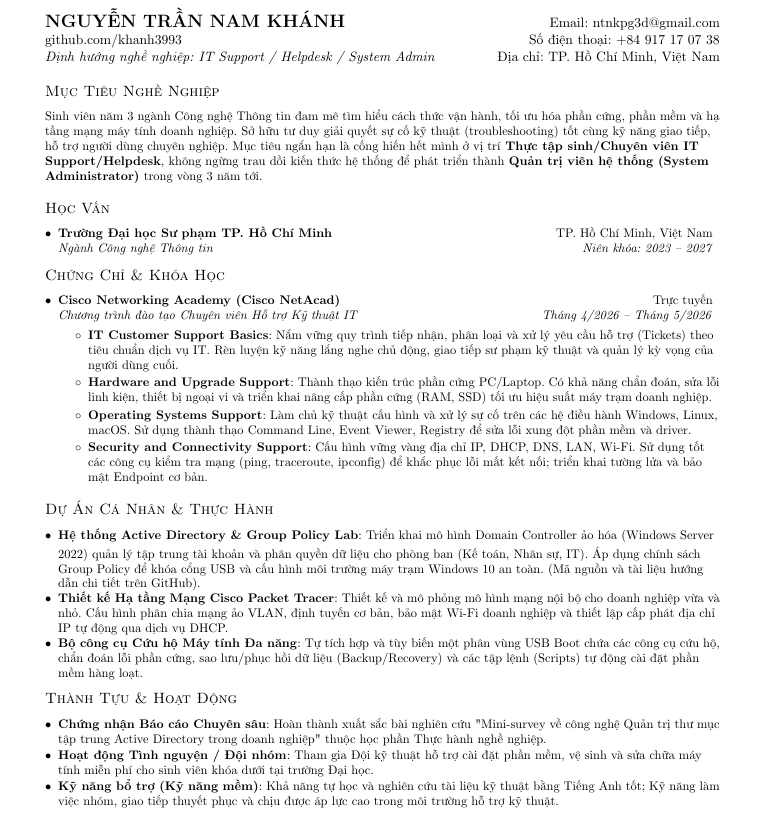
\includegraphics[width=6.1in,height=6.56667in]{./media/image2.png}

\textbf{6.2 Portfolio cá nhân}

\begin{itemize}
\item
  Link website cá nhân:
  \href{https://khanh3993.github.io/}{\textbf{khanh3993.github.io}}
\item
  Quá trình thực hiện:

  \begin{itemize}
  \item
    Phát triển mã nguồn: Trang web được xây dựng thủ công bằng HTML5 và
    CSS3 với giao diện tối giản, hiện đại và hỗ trợ hiển thị tốt trên
    nhiều thiết bị (Responsive Design).
  \item
    Quản lý dự án: Tôi đã sử dụng tệp README.md để viết mô tả chi tiết
    về cấu trúc trang web và hướng dẫn quy trình triển khai bằng GitHub
    Pages để người khác có thể tham khảo.
  \item
    Nội dung Portfolio: Trang web bao gồm đầy đủ các mục bắt buộc: Giới
    thiệu cá nhân, Các dự án tiêu biểu, Danh sách chứng chỉ và Thông tin
    liên hệ chuyên nghiệp.
  \end{itemize}
\end{itemize}

\textbf{Chương 7:} Hồ sơ LinkedIn cá nhân

LinkedIn là mạng xã hội nghề nghiệp lớn nhất hiện nay và là công cụ
không thể thiếu để xây dựng thương hiệu cá nhân, kết nối với cộng đồng
IT và tiếp cận các cơ hội việc làm. Nhận thức được tầm quan trọng đó,
tôi đã chủ động xây dựng và hoàn thiện hồ sơ LinkedIn chuyên nghiệp.

\textbf{7.1 Thông tin hồ sơ}

\begin{itemize}
\item
  Đường dẫn Hồ sơ LinkedIn cá nhân:
  \href{https://www.linkedin.com/in/kh\%C3\%A1nh-nguy\%E1\%BB\%85n-975b48326/}{Khánh
  Nguyễn \textbar{} LinkedIn}
\end{itemize}

\textbf{7.2 Các hạng mục đã hoàn thiện}

Để hồ sơ thể hiện rõ ràng năng lực và định hướng trở thành Fullstack Web
Developer, tôi đã cập nhật đầy đủ 04 hạng mục quan trọng nhất:

\begin{itemize}
\item
  Giới thiệu bản thân (About): Trình bày tóm tắt về nền tảng học vấn tại
  trường Đại học Sư phạm TP. Hồ Chí Minh (HCMUE), định hướng chuyên sâu
  vào mảng IT Support và thái độ cầu tiến trong công việc.
\item
  Kỹ năng chuyên môn (Skills): Bổ sung và phân loại các kỹ năng cốt lõi
  bao gồm công cụ quản lý mã nguồn (Git/GitHub), và quản trị hệ thống
  (Ubuntu/Windows Server).
\item
  Chứng chỉ (Certifications): Liên kết trực tiếp các chứng chỉ trực
  tuyến đã đạt được từ Cisco. Các chứng chỉ này được xác thực ID rõ
  ràng, minh chứng cho năng lực tự học.
\item
  Dự án thực tế (Projects): Cập nhật thông tin chi tiết về các dự án cá
  nhân.
\end{itemize}

\textbf{Chương 8:} Tự đánh giá \& định hướng tiếp theo

Sau giai đoạn học tập và thực hành nghề nghiệp giữa kỳ, tôi đã có cái
nhìn rõ nét hơn về năng lực bản thân so với yêu cầu thực tế của ngành
Công nghệ thông tin. Chương này trình bày những đánh giá chủ quan và kế
hoạch hành động trong thời gian tới.

\textbf{8.1 Điểm mạnh}

Khả năng tự học và thích nghi công cụ: Tôi đã làm chủ được các công cụ
kỹ thuật chuyên sâu như LaTeX và Git trong thời gian ngắn, đồng thời
hoàn thành các chứng chỉ trực tuyến từ Cisco.

Quản lý công việc khoa học: Sử dụng hiệu quả hệ sinh thái Google
Workspace để lên lịch trình và theo dõi tiến độ học tập.

\textbf{8.1.2 Điểm yếu và kỹ năng cần cải thiện}

Thiếu kĩ năng: Hiện tại, khả năng của tôi chỉ mới ở bước entry-level
(căn bản), tôi cần phải học thêm nhiều kĩ năng khác liên quan đến mạng
(CCNA 200-301).

Ngoại ngữ chuyên ngành: Cần cải thiện vốn tiếng Anh chuyên sâu để có thể
đọc hiểu tài liệu kỹ thuật nhanh chóng và tham gia các diễn đàn công
nghệ quốc tế.

Kiến thức về Cloud: Do rào cản về phương thức thanh toán, tôi chưa thực
hành sâu trên Google Cloud/AWS, đây là mục tiêu trọng tâm cần khắc phục
trong giai đoạn tới.

\textbf{PHỤ LỤC}

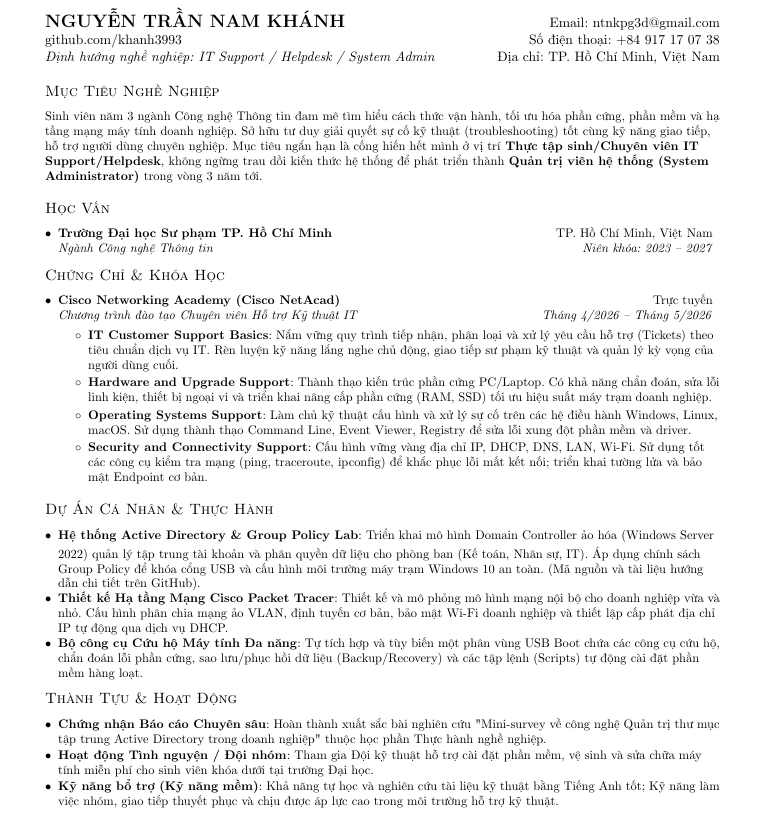
\includegraphics[width=6.1in,height=6.56667in]{./media/image2.png}

Hình 1: Ảnh chụp màn hình cv.pdf/tex

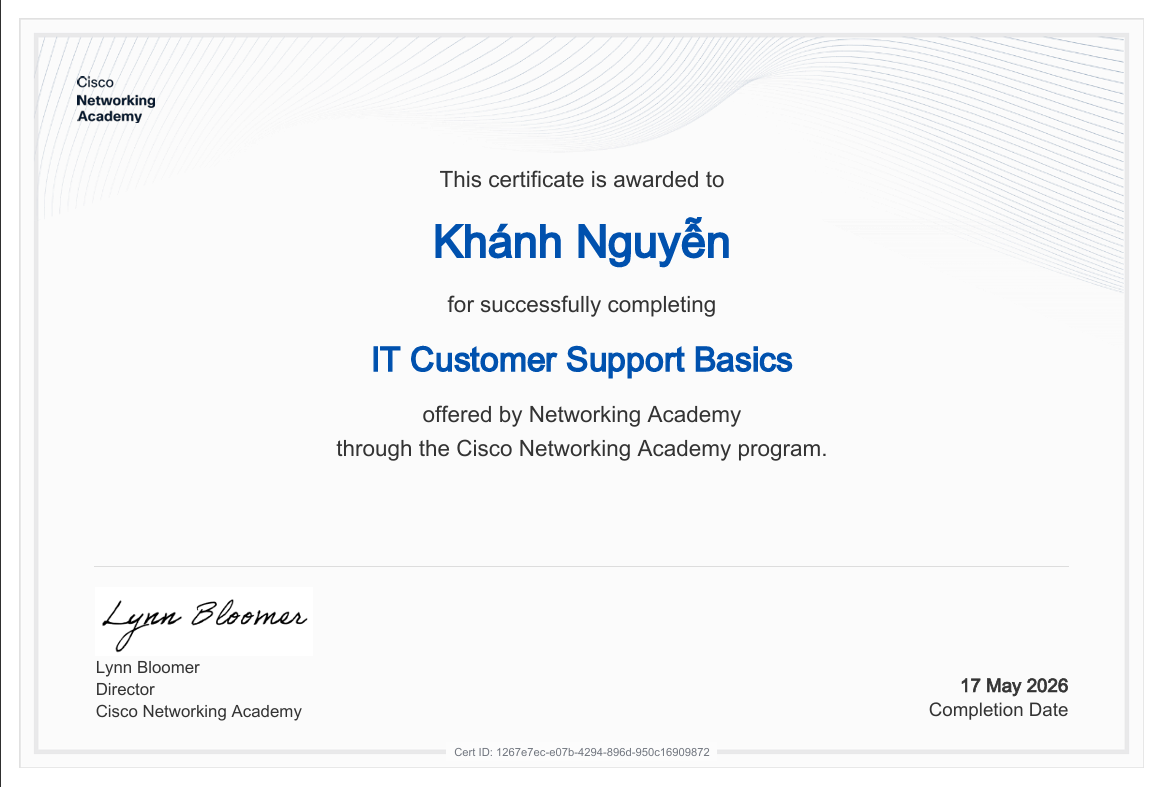
\includegraphics[width=6.1in,height=4.13333in]{./media/image3.png}

Hình 2: Ảnh chụp màn hình chứng chỉ IT Customer Support Basics

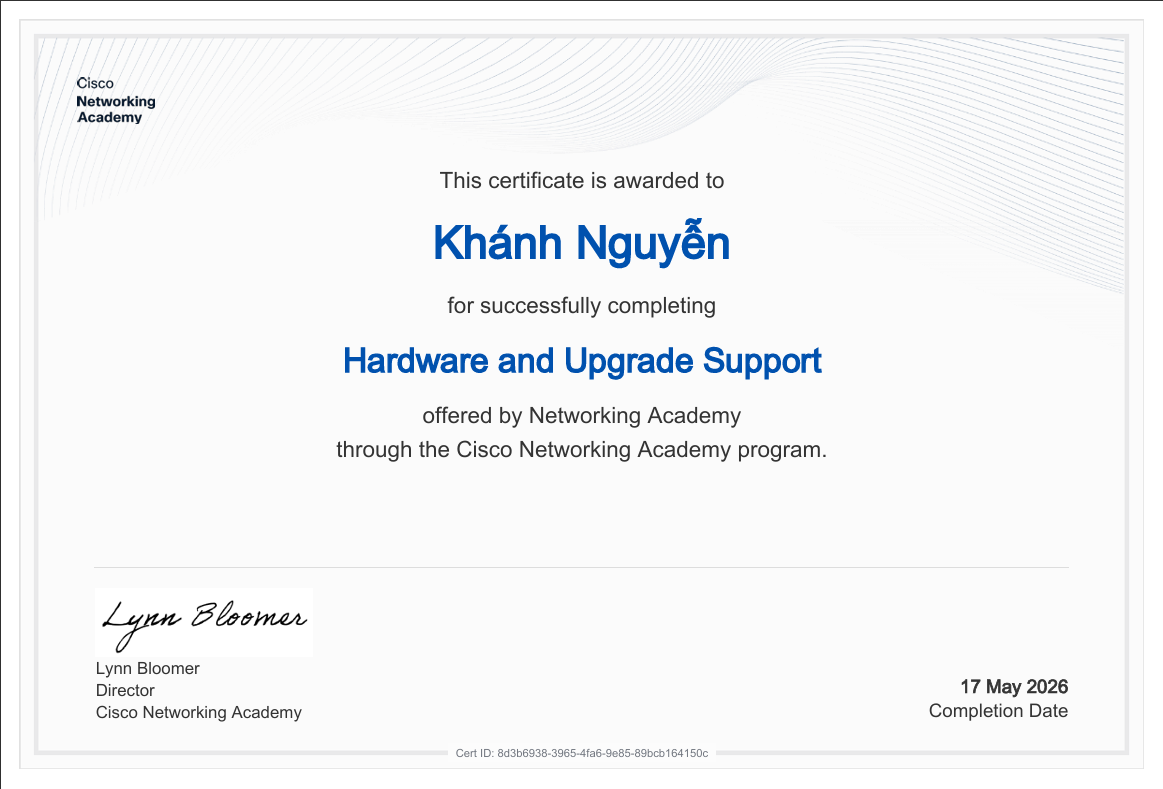
\includegraphics[width=6.1in,height=4.13333in]{./media/image4.png}

Hình 3: Ảnh chụp màn hình chứng chỉ Hardware and Upgrade Support

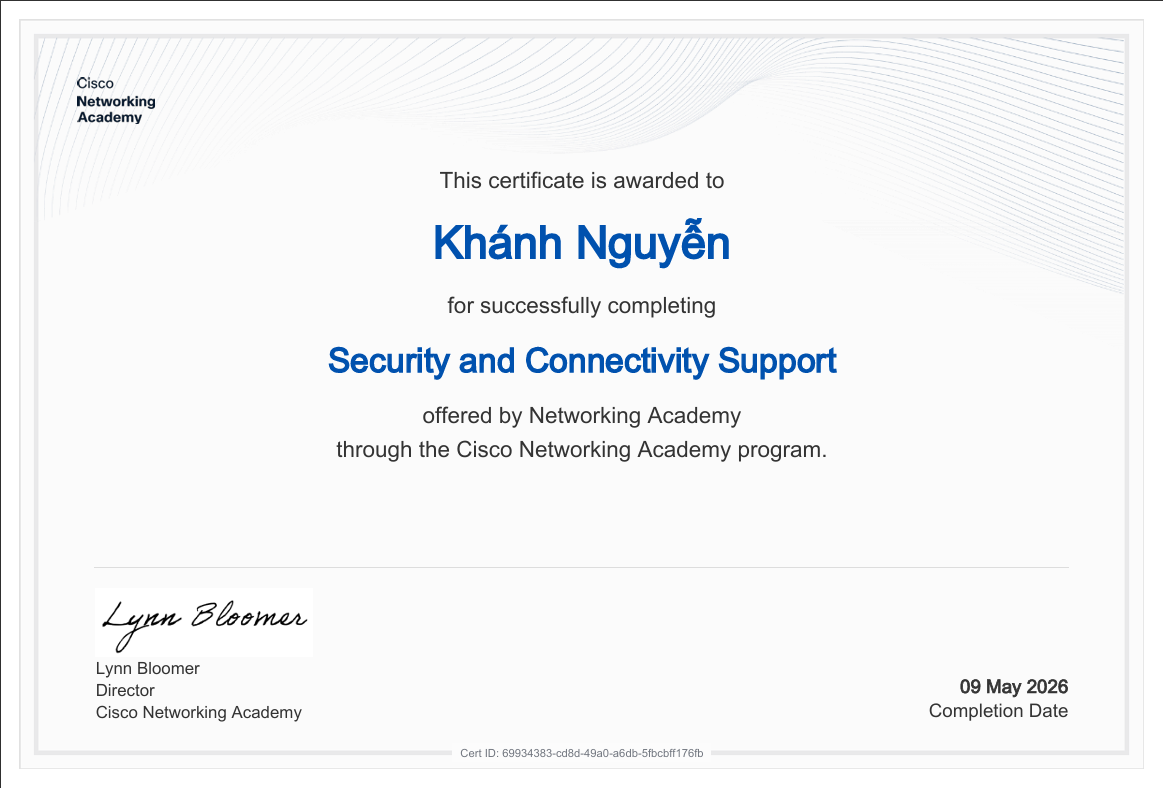
\includegraphics[width=6.1in,height=4.13333in]{./media/image5.png}

Hình 4: Ảnh chụp màn hình chứng chỉ Security and Connectivity Support

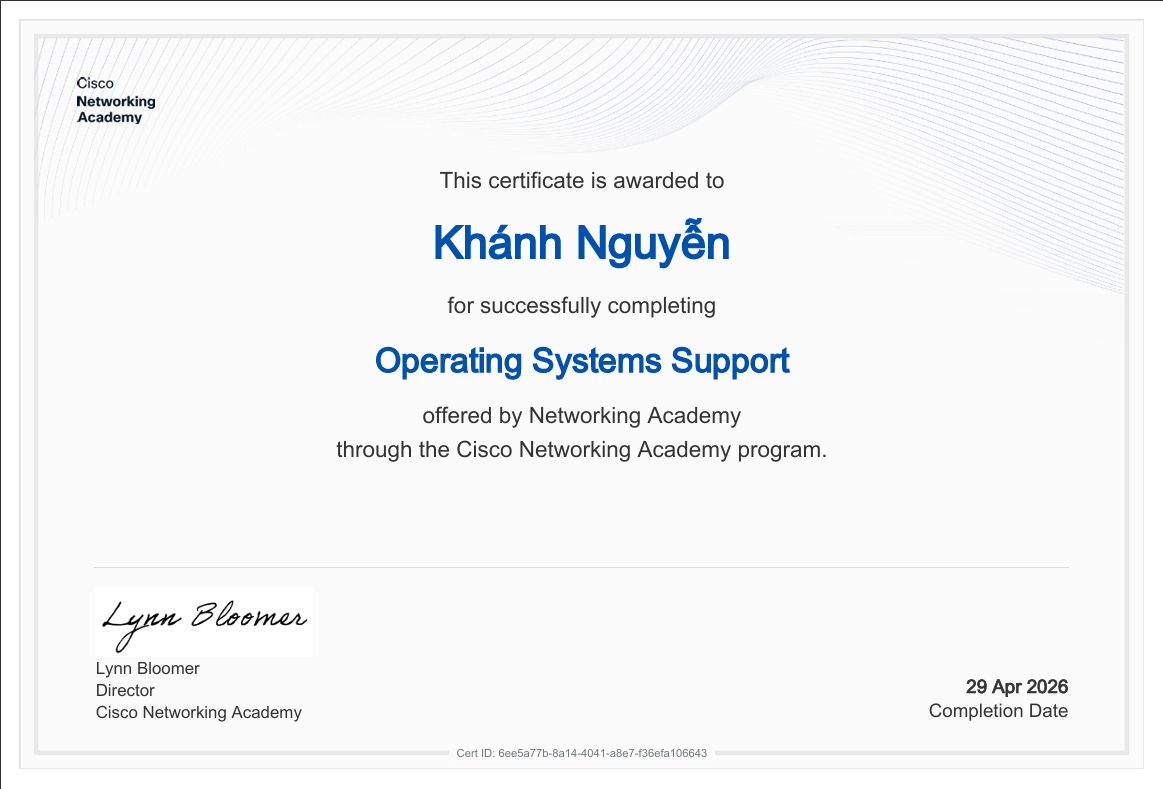
\includegraphics[width=6.1in,height=4.13333in]{./media/image6.png}

Hình 5: Ảnh chụp màn hình chứng chỉ Operating Systems Support

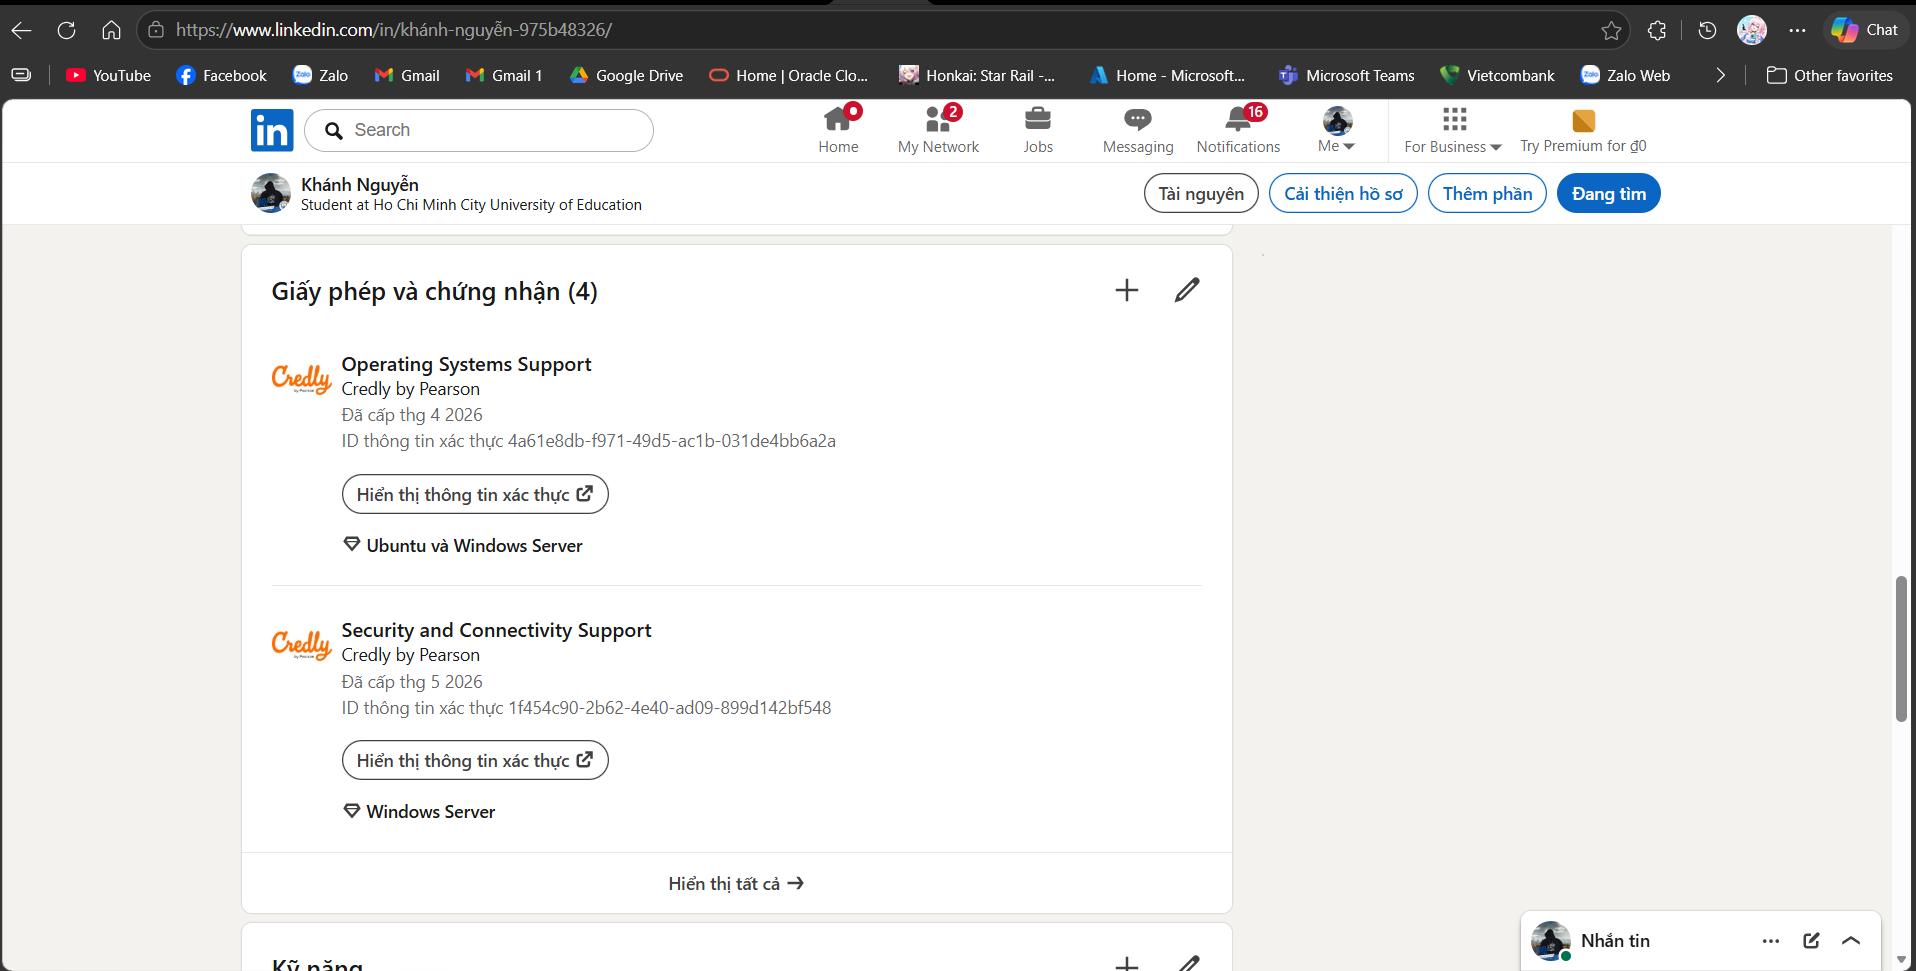
\includegraphics[width=6.1in,height=3.09167in]{./media/image7.png}

Hình 6: Ảnh chụp màn hình LinkedIn cá nhân

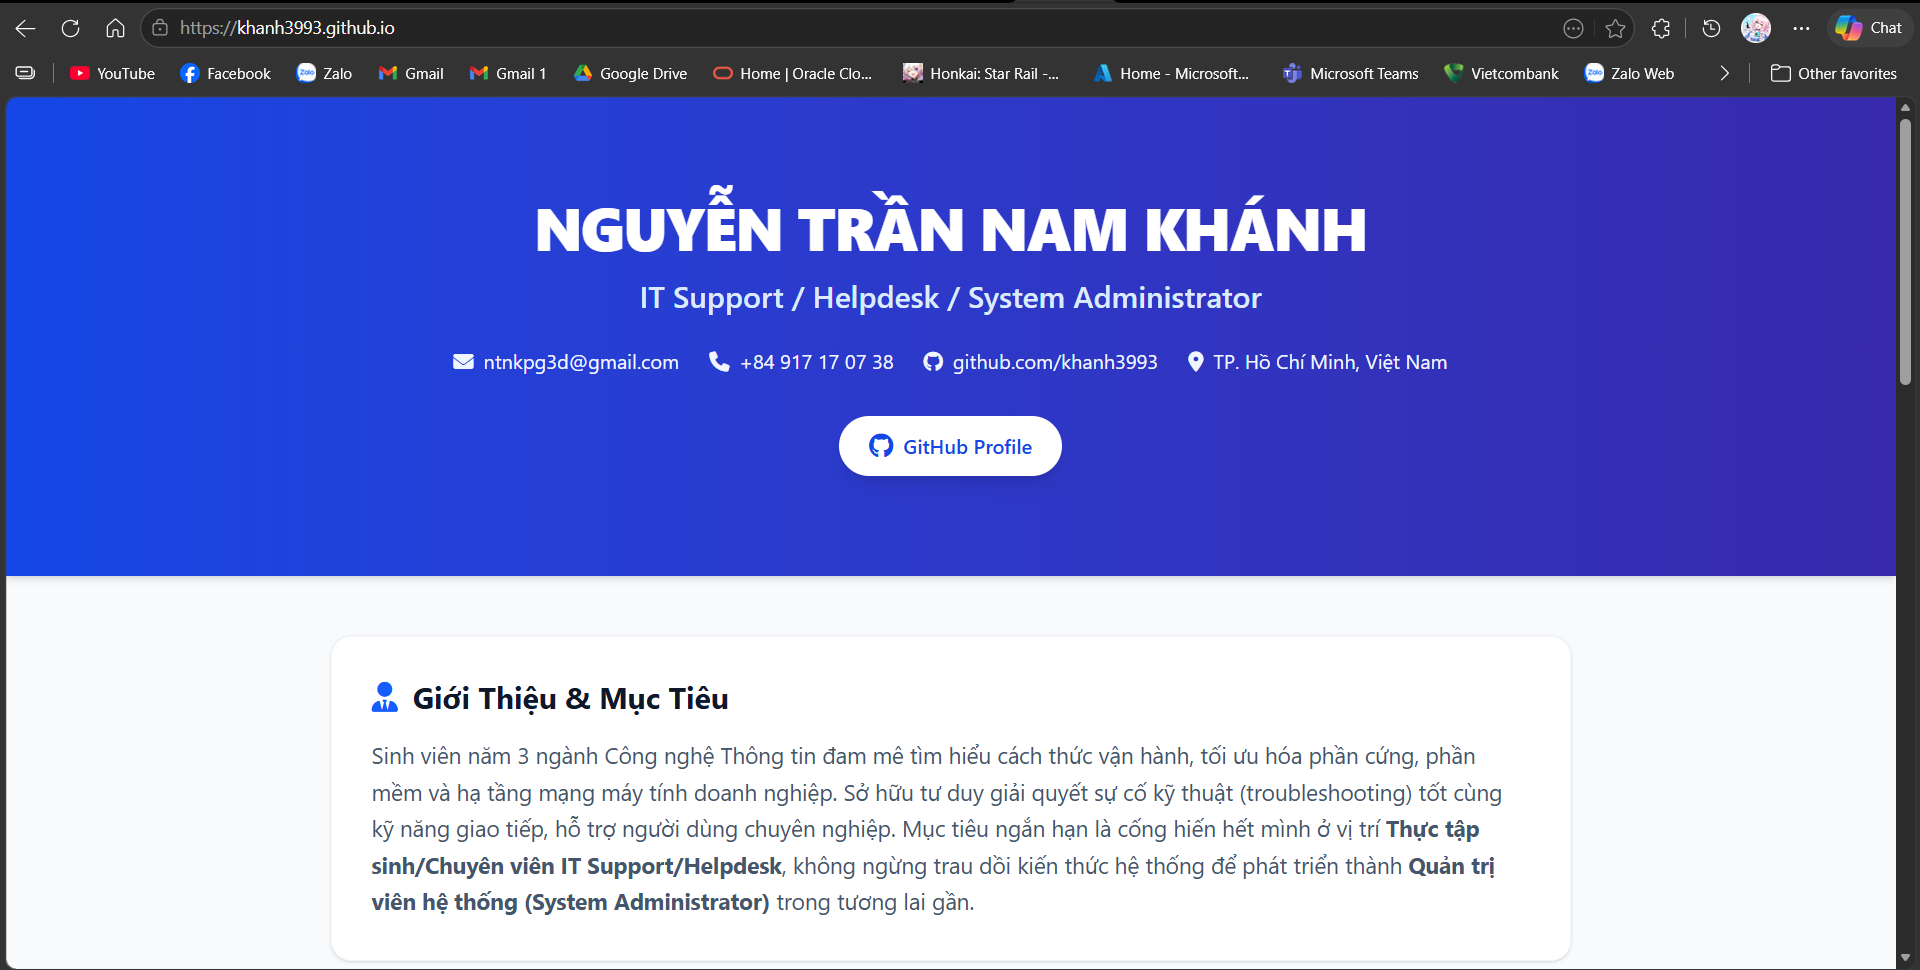
\includegraphics[width=6.1in,height=3.08333in]{./media/image8.png}

Hình 7: Ảnh chụp màn hình Github Page

\end{document}